\chapter{Implementation}

\TODO{intro to implementation}


\section{Navigation}

\subsection{First Person Mode}

This navigation mode is centered on the current point of view and works by triggering the displayed gates.
It features 8 gates: 4 direction displacement gates and 4 rotation gates.
To stop the movement/rotation one can either trigger the gate again, effectively disabling the ongoing action
or by triggering a different gate action.

The choice for this mode's layout suffered several evolutions.
At early stages opposing directions where placed at opposite sides of the ring but this
made correction by triggering the opposite action difficult, so opposing actions are now close together.
In this mode a restriction of one enabled action at a time is imposed to keep the handling easy for novice users
there as soon as an action starts the previous one stops.

There are gates for moving forward/backwards, up/down, pitch up/down and yaw up/down
\footnote{The verbs pitch and yaw come from flight semantics: to pitch is to look up/downwards; to yaw is to turn relatively to the ground plane.}.

\TODO{FIGURE}


\subsection{Compass Mode}

The compass mode was thought out for searching tasks. It allows the user to move along the ground plane and turn around it.

The compass navigation mode has 2 distinct areas:
the center circle displays a top-down view of the scene centered on the user;
the outer ring displays the main compass directions.

In order for one to move a drag must be performed inside the top-down view.
To reorient the user one must rotate the outer ring. The direction the user is facing can be read on the top part of the ring.

This mode could not be tested on multi-screen displays due to technical problems. It was enthusiastically accepted on
one-projector early tests.

\TODO{FIGURE}


\subsection{Examine Mode}

The examine mode allows the user to recenter attention on an object of the scene.
It features 3 gates and a center sphere.
The user must initially select the new center of attention, by triggering the recenter gate,
finishing the stroke at the desired object/location.
Once the location is defined the remaining gates allow for zooming in and out the content
while the sphere allows for repositioning the user on the space around the object -- 
horizontal moves rotate horizontally, vertical moves vertically.

This mode is the most effective when performing shape modeling tasks.

\TODO{FIGURE}


\section{Content Creation}

The system's interface offers 3 families of shapes which can be instanced on the scene.
There are the primitives cube, cylinder and sphere; a set of previously generated shapes
and set of known building styles from which one can create buildings.
The primitives are the most versatile shapes since they support face and edge manipulation operations.
All shapes support simple transformations and cloning.

One uses building styles to create buildings on the scene, the library of generated shapes such as
people, trees and other asserts to populate the scene with such details and the primitives as is or as
building ground for custom shapes.

\TODO{FIGURE SHAPE MENU}


\subsection{Shape Instancing}

The instancing of shapes works using the Apply-to-Scene concept \TODO{GET REF}.
Every gate of this type has a small arrow running outwards as a hint to the user of the feature.
The user activates the gate of the desired shape and ends the stroke where he wants it to rest.

\TODO{EXAMPLE IMAGE}


\subsection{Building Instancing}

\TODO{ADD CALI TO BLOCKS, HERE AND TRIANGLE STROKE}
Once the building parameters have been gathered by the interface, as described on \TODO{GET REF},
the building needs to be generated.
First the stroke is projected onto the construction plane and parsed by the shape recognizer as a rectangle.
Its dimension serve as the blueprint which is extruded upwards for the measured height.
Then the building facades are generated according to the chosen style grammar and so is the ceiling.
The style grammar is fed each facade length and returns a set of spacings and facade elements that must be instanced
according to the rules defined in the style.
If for instance the facade rule for a given floor says
``center a door and use windows everywhere else'' the system measures the width of both door and window and returns
the maximum number of windows and a door in the center that fit the facade.
To minimize the facade attachments in memory, a map of loaded attachments is managed so only the first instance of any
attachment is loaded.


\subsection{Building Style Grammar}

\subsubsection{Grammar Structure}

The building style grammar defines building parameters such as
\textbf{floor-height}, \textbf{ceiling} parameters and \textbf{color-interval}s for the walls and ceiling.
It also defines a set of rules for the generation of the facade attachments that make up the final facades,
defined by the optional \textbf{front-facade} and the \textbf{facades} elements.

One can define the layout of a floor with the \textbf{layout} element, composed of 4 sections:
\textbf{left}, \textbf{center}, \textbf{right} and \textbf{other}.
Only the \textbf{other} section is required and the layout works by trying to fill the facade space with \textbf{center}, \textbf{left} and \textbf{right}s' contents if those are present, repeating \textbf{other}'s contents for filling the remaining space.

Inside these sections one can put the any of the \textbf{us-element}s: \textbf{atom}, \textbf{group}, \textbf{sequence} and \textbf{random}.
An \textbf{atom} is the simplest \textbf{us-element}, having the attributes
\emph{type}, \emph{spacing} and \emph{height}.
The \emph{type} parameter defines which shape to instantiate on the facade,
\emph{spacing} how many width it will consume and
\emph{height} can be used to shift the shape upwards (to move a window, for instance).

The remaining \textbf{us-element}s allow combining \textbf{us-element}s.
A set of \textbf{us-element}s inside a \textbf{group} instance all content on the same place and measure the longest of its children.
A set of \textbf{us-element}s inside a \textbf{sequence} instance all children one after the other.
The \emph{random} \textbf{us-element} is similar to \textbf{group}, but has the attribute \emph{odds},
a set of comma separated ratios defining the probability of the children to be picked.

Several floors can share the same layout. To apply a layout to one or a set of floors, the floor-span element exists.
It can have either the \emph{at} attribute defined or both \emph{min} and \emph{max},
resulting in the application of the enclosed layout to all the floors in the interval.

One can also define a different facade style for the front facade with the element \textbf{front-facade}.
This is useful when one wants to apply columns and doors to one facade but not the remaining ones.


%It is defined on the XSD document for reference.


%\input{grammar.tex}

\subsubsection{Grammar Example: Residential Style}

notation and examples

\section{Content Editing}

\subsection{Face Selection}

\subsection{Edge Selection}

\subsection{Direction Election}

\subsection{Shape Structure and Operations}




\section{Reviewing}

\section{Proposed Work Flow}


%\TODOL{IMMIVIEW OVERVIEW?}
%\section{ImmiView Framework}

\subsection{Architecture}


%\section{General Interface}

\subsection{Strokes}

A \emph{stroke} is a continuous set of points drawn on our system.
Since the system works both on Tablet PCs and on power walls,
a stroke can be drawn either with the tablet's pen or with
a regular laser pointer.

Drawing strokes is therefore the main way of users interaction with
the system. It has been built to support several users interacting
simultaneously in the screen.

With this approach, any component in the system can't make use
of global mode information due to the fact that one can't know
for sure if the $ stroke_{n+1} $ was drawn by the same user than $ stroke_{n} $.

Therefore, strokes must serve many purposes, and in cases where a sequence
of actions must be done in order, they're achieved under the same stroke.

Another decision taken early on in the implementation was that there shall not be
fixed areas in the screen for contents such as menus. The initial state of the
system is completely free of interface widgets. When starting the system the users
see only a 3D perspective of the virtual world.


\subsubsection{Stroke Actions}

Any stroke can be interpreted as being one of (see figure \ref{fig:lasso-tri}):

\begin{description}
		\item[an open stroke] --
				any stroke where the segments don't intercept each other;

		\item[a lasso] --
				a closed stroke;

		\item[a triangle stroke] --
				this is a special case of a lasso, i.e. closed, where the stroke resembles a triangle.
\end{description}


\begin{figure}[!ht]
		\centering
		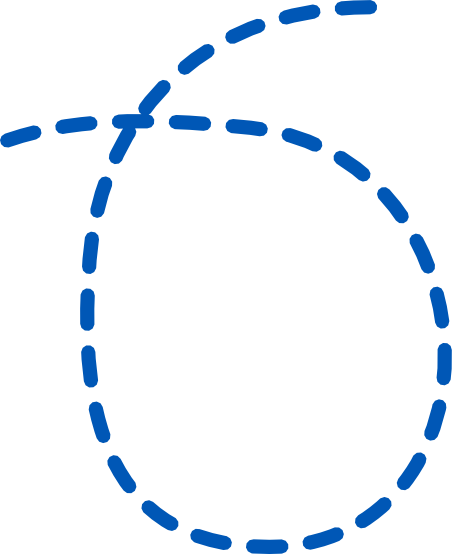
\includegraphics[width=3.5cm]{gfx/lasso.png}
		\qquad\qquad\qquad
		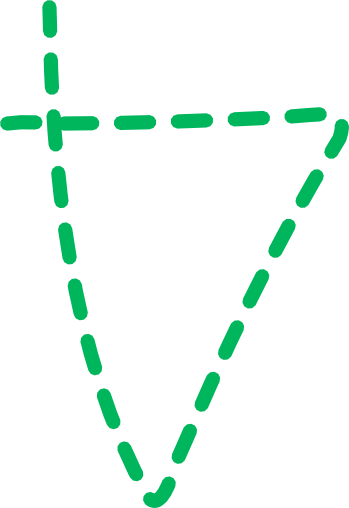
\includegraphics[width=3cm]{gfx/triangle.png}
		\caption{Lasso and triangle strokes}
		\label{fig:lasso-tri}
\end{figure}


\subsection{Gates}

As described earlier on in section \ref{sec:gate-concept} The Gate Concept,
a gate solves the problem of our input devices not being capable of detecting
click actions consistently.

\begin{figure}[!ht]
		\centering
		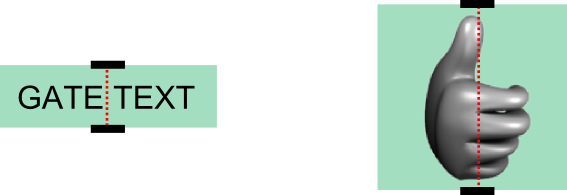
\includegraphics[width=5cm]{gfx/gate1e.png}
		\vspace{-0.5cm}
		\caption{Two gates: one featuring text and the other visual content}
		\label{fig:gate1}
\end{figure}

\begin{figure}[!ht]
		\vspace{-0.7cm}
		\centering
		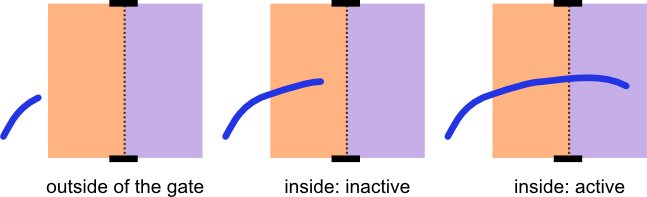
\includegraphics[width=10cm]{gfx/gate2e.png}
		\vspace{-0.5cm}
		\caption{Gate activation}
		\label{fig:gate2}
\end{figure}

\begin{figure}[!ht]
		\vspace{-0.7cm}
		\centering
		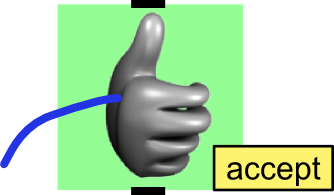
\includegraphics[width=3cm]{gfx/gate3e.png}
		\vspace{-0.5cm}
		\caption{Gate showing its tooltip}
		\label{fig:gate3}
\end{figure}


Gates can either have text our visual content (fig \ref{fig:gate1}).
It was decided that gates shouldn't feature both at the same time.

The activation takes place by entering both the left side and the right
side areas of the gate consecutively (or the other way around).
The dashed line in figure \ref{fig:gate2} is only imaginary.

In order for users to inspect the meaning a gate with visual content, a
tooltip appears when the stroke is inside the gate,
which will happen prior to activation, so users can give it up (figure \ref{fig:gate3}).

In conclusion, for a user to activate a gate, an horizontal or quasi-horizontal
stroke must be drawn, as seen in figure \ref{fig:gate4}.

\begin{figure}[!ht]
		\centering
		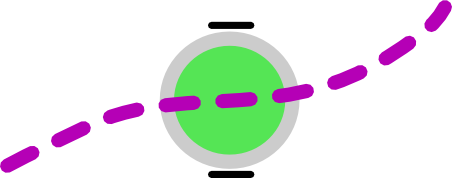
\includegraphics[width=4cm]{gfx/activation.png}
		\caption{gate activation example}
		\label{fig:gate4}
\end{figure}

\subsection{Menus}

In order to get the main menu, the user has to draw a closed triangle stroke.
The menu appears at the center of the drawn stroke.

\begin{figure}[!ht]
		\centering
		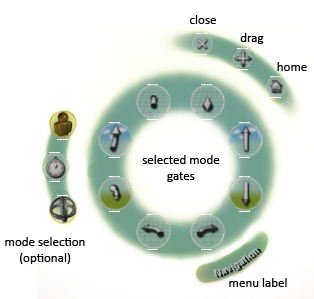
\includegraphics[width=8cm]{gfx/menu.png}
		\caption{menu and its components}
		\label{fig:menu}
\end{figure}

Menus are round and have additional auxiliary gates and labels (figure \ref{fig:menu}).

In the bottom right area a label clearly identifies the functionality provided by the menu.

In the top right area menus feature a set of special gates.
The \emph{close gate} dismisses the menu.
The \emph{move gate}, when activated, makes the menu follow the stroke position until it ends.
The \emph{home gate} allows the user to go back to the previous menu, when that action applies.

Occasionally the menus are too complex and need to be segmented.
When that happens, mode selection gates appear to the left of the menu.

Different menus have different background colors.
They're translucent so the main perspective remains partially visible.
Menu colors were chosen to reflect the functionality, ex: all navigation menus are green.


%
\section{Navigation}

\subsection{1st Person Navigation Mode}

\TODO{ADD 1ST PERSON SHOT}
This widget has four moving directions and four rotations.
It allows to move forward/backward,
go up/down,
turn left/right and
pitch up/down.

Crossing a gate once starts the movement.
Crossing it again stops it.
If a gate is crossed while another one is active,
the first one stops -- this behavior was enforced
by user test inspection.
Having several moving/rotation
actions applied at the same this is confusing.
Clarity was favored over efficiency.

\subsection{Compass Navigation Mode}

\TODO{ADD COMPASS SHOT}

This is a direct application of the concept defined
in section \ref{sec:bev} Bird's Eye View Mode, on page \pageref{sec:bev}.

The outer ring of the widget allows the user to see and change
the current orientation in terms of cardial points positioning.

The inner circle allows inspection of the top-down view, with the user
being in the center. Applying strokes inside this area drags the map,
changing user's position in the ground plane.

\subsection{Examine Navigation Mode}

\TODO{ADD EXAMINE SHOT}

\TODO{ADD VIRTUAL SPHERE ILLUSTRATION}

This widget features a wire frame sphere at the center, two zooming gates
and two additional gates whole purpose is described below.
It is a direct application of the concept defined
in section \ref{sec:examine} Examine Navigation Mode, on page \pageref{sec:examine}.

The sphere occupying the center of the widget simulates the virtual sphere centered
on the subject of interest with radius $ dist $.

The user is at distance $ dist $ from the subject of interest.
This distance can be increased or decreased by activating the zoom gates.
Movements in the $ XX $ direction are translated into rotations around $ \theta $, while
movements in the $ YY $ direction translate into rotations around $ \phi $.

Two additional gates allow changing the subject of interest.
They work by crossing and ending the stroke at the target.
The first one, \emph{point of interest center}, allows one to examine the center of the object.
The remaining one, \emph{point of interest spot}, changes the examined position to be the surface
position where the stroke ``touches''.
The former is useful for inspection of the overall object while the latter is of great
use in editing or inspecting surface details.

\subsection{Fly Navigation Mode}

%intro DONE

\begin{figure}[!ht]
		\centering
		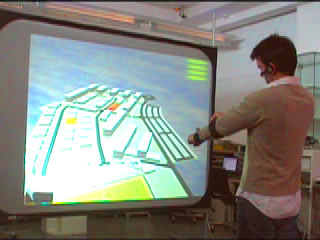
\includegraphics[width=6cm]{gfx/don.png}
		\caption{user navigating with the multimodal navigation mode}
		\label{fig:don}
\end{figure}

Navigation in a 3D scene takes place normally using a desktop computer
with the mouse and keyboard as input devices and the monitor as output device.
In the multimedia lab there was a motion tracking system available.
It was put to use in conjunction with a wireless microphone to allow for an
alternative mode of navigation. A set of reflective markers is attached to
the user's arms and the wireless microphone attached to his/her ear.
The microphone allows for enabling and disabling the multimodal navigation mode
by issuing respectively the commands \textbf{begin flying} / \textbf{stop flying}.

\subsubsection{Physical Configuration}

Motion tracking took place using reflective markers attached to the user's arms (figure \ref{fig:markers-cams} left).
A set of 4 cameras with infrared lights were installed in the lab, which each
captured image being processed by a computer identifying the visible markers in
image-space, making the computation of the spacial position of each marker by
merging the data from the 4 captured views and labeling each tracked marker
from the initial extended arm pose (figure \ref{fig:markers-cams} right).

The Microsoft Speech API 5.1, American English version was used to recognize the
voice commands. Capturing of the commands was done by attaching a wireless microphone
to the user's ear.

%ap�s a compara��o do reconhecimento do mesmo face a um microfone fixo e um Bluetooth.

%O reconhecedor mostrou-se algo limitado, tendo sido necess�rio adaptar a gram�tica a palavras n�o amb�guas entre si ou
%que gerassem falsos positivos.
%
%%Preliminarmente realizou-se um teste para escolher o melhor hardware para reconhecimento de voz, entre um microfone Wireless, %um fixo a captar toda a sala e um auricular Bluetooth. Os comandos dispon�veis na aplica��o foram ditados repetidas vezes por 3 %utilizadores, em ordem aleat�ria e com os 3 dispositivos.
%
%%Conclui-se que o microfone Wireless era a melhor op��o com uma taxa de reconhecimento m�dia de 99\%, mas para dist�ncias curtas %(\(<\)3m) o auricular Bluetooth teve resultados semelhantes, com 98\%. O microfone fixo captou muito ru�do e produziu resultados %muito insatisfat�rios de menos de 50\%.

%O reconhecedor mostrou-se algo limitado, tendo sido necess�rio adaptar a gram�tica a palavras n�o amb�guas entre si ou
%que gerassem falsos positivos.

\begin{figure}[!ht]
		\centering
		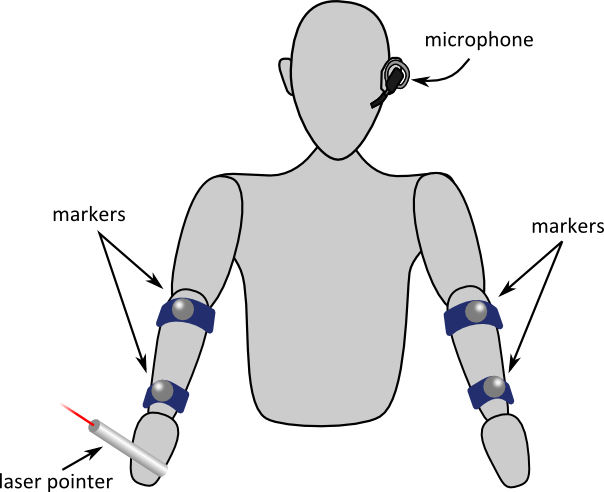
\includegraphics[width=7cm]{gfx/markers2.png}
		\qquad
		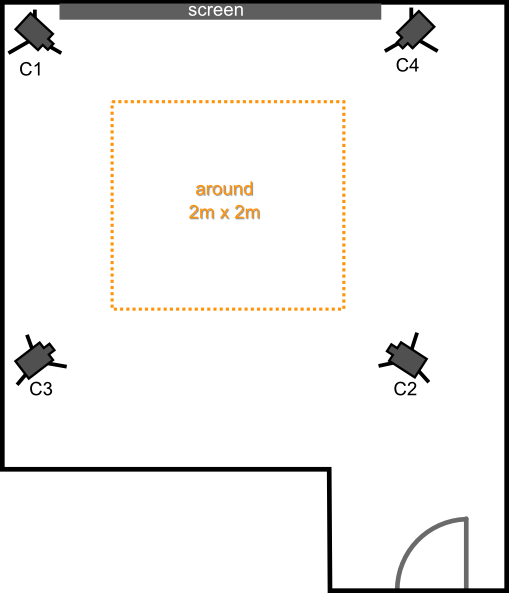
\includegraphics[width=5cm]{gfx/4cam-setup.png}
		\caption{markers and camera setup}
		\label{fig:markers-cams}
\end{figure}
%
%
%\begin{figure}[!ht]
%		\centering
%		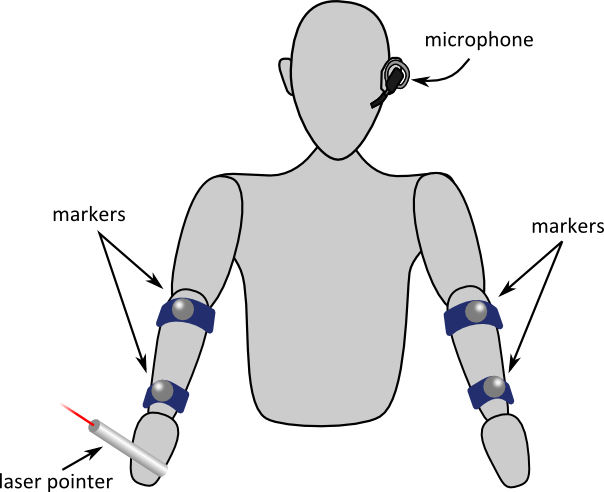
\includegraphics[width=6cm]{gfx/markers2.png}
%		\caption{markers and microphone for tracked user}
%		\label{fig:markers}
%\end{figure}
%
%\begin{figure}[!ht]
%		\centering
%		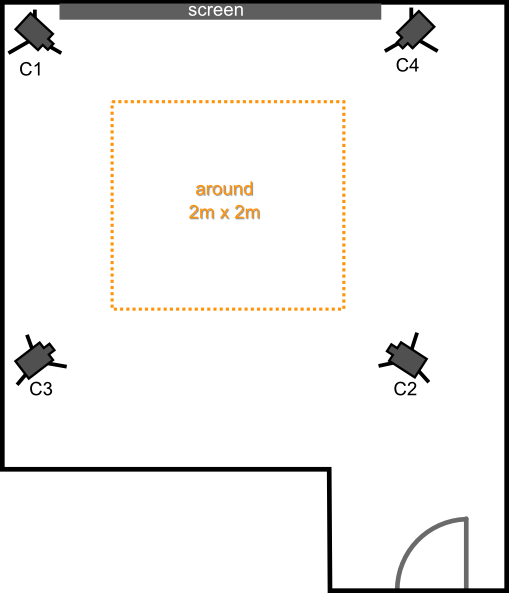
\includegraphics[width=6cm]{gfx/4cam-setup.png}
%		\caption{four cameras setup for motion tracking}
%		\label{fig:cam-setup}
%\end{figure}


\subsubsection{Interaction}

The multimodal navigation mode requires the user to have his / her arms extended towards the screen.

Controlling the flight speed works by the measurement of the distance between hands:
the closer they are from each other, the faster the flight speed is.
If the arms get close to a ninety degrees angle between them the flight halts (figure \ref{fig:fly-speed}).

Changing the flight orientation relatively to the ground plane is achieved by setting the arms
angle with the ground at opposing directions, with a bigger difference between angles generating
a faster rotation movement. If the user wants to turn right, for instance, he / she has to
raise the left arm and lower the right one (figure \ref{fig:fly-rot-up}, left).

To change flight altitude, both arms must be oriented in the same direction relatively to the ground plane,
either both raised or both lowered.
Again, the higher the angle is from the original arms extended forward pose,
the bigger the flight altitude shift occurs (figure \ref{fig:fly-rot-up}, right).

\begin{figure}[!ht]
		\centering
		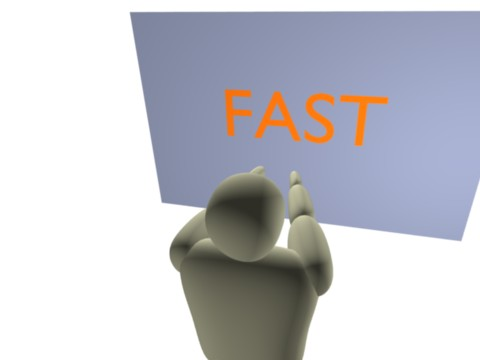
\includegraphics[width=5cm]{gfx/immi-fly-fast.jpg}
		\qquad
		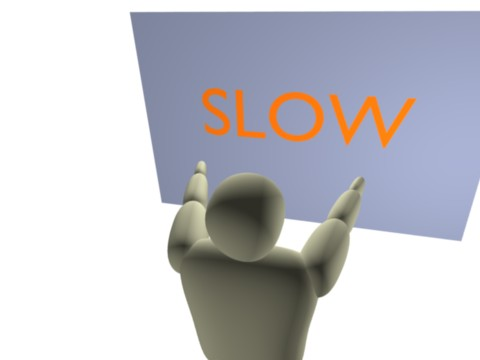
\includegraphics[width=5cm]{gfx/immi-fly-slow.jpg}
		\caption{control flight speed}
		\label{fig:fly-speed}
\end{figure}

\begin{figure}[!ht]
		\centering
		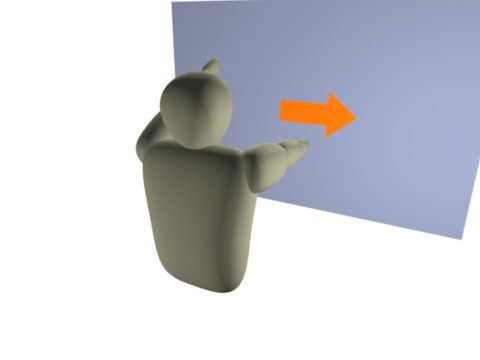
\includegraphics[width=5cm]{gfx/immi-fly-rotate.jpg}
		\qquad
		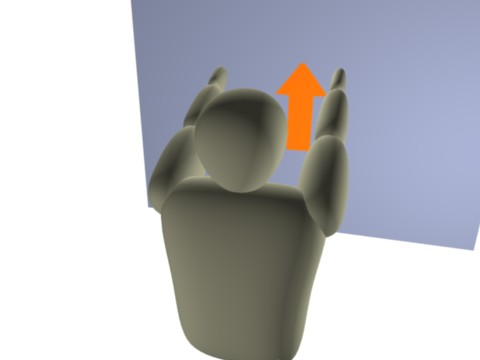
\includegraphics[width=5cm]{gfx/immi-fly-up.jpg}
		\caption{rotate flight orientation and increasing flight altitude}
		\label{fig:fly-rot-up}
\end{figure}

%
%\TODO{IMMI PAPER}


%
\section{Building Creation}

\section{Custom Shape Creation}

\TODO{CV PAPER}


%
\section{Custom Shape Creation}

The purpose of this functionality is to grant the user a simple yet robust shape
structure supporting a set of geometry transformation operations,
so that custom shapes can be modeled with ease. Figure \ref{fig:example} shows an example result.

\begin{figure}[!ht]
	\centering
	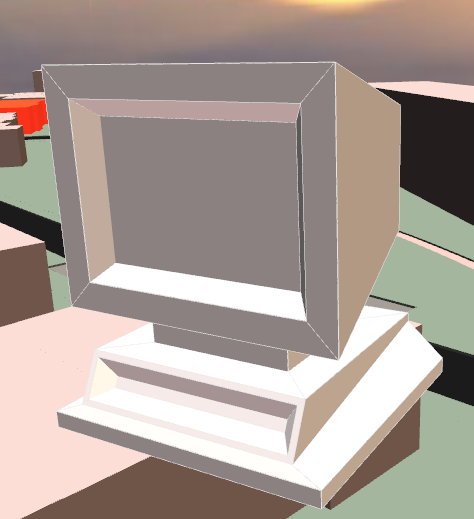
\includegraphics[width=5cm]{gfx/ex-monitor.png}
	\caption{monitor shape modeled in the system}
	\label{fig:example}
\end{figure}

\subsection{Internal Structure}

The defined structure to support the custom shape is based on 4 sided faces.
This decision implies that:
\begin{itemize}
	\item every edge is shared by two faces;
	\item every edge in a face has an opposite edge relating to that face.
\end{itemize}

Besides the \emph{list of vertices} and its positions and the \emph{list of faces}
(each face being a list of 4 vertex indices),
an additional structure is computed: the \emph{edge map}.
It maps which faces share each edge.
This information is used to optimize the low-level operations for
getting the opposite edge and getting the face loop,
a	paramount to the split face loop operation.

Aside from these data structures which hold the shape's form,
there's a \emph{list of face colors}, one per face, to hold the shape's appearance.

These shapes support the undo operation. It was implemented based on the Memento design pattern \cite{despat}.
Each object has an associated stack of states, so the user can return to any previous state of modeling if needed.


\subsubsection{Persistence}
\label{sec:shape-persistence}

Each modeled object is responsible for saving its geometry data.
The chosen format for persistence was XML and each shape is translated into an XML element.

The format resembles the simplified structure of a WaveFront OBJ file, but described in XML.
The vertices are listed, starting from index 0.
Next each face is defined as an ordered list of 4 vertex indices.
The list of colors, one for each of the faces, is described in the end.

\begin{small}
	\begin{verbatim}
	<?xml version="1.0" encoding="utf-8"?>
	  <shape>
	    <vertices count="56">
	      <vertex x="-1" y="-0.627882" z="5.29942"/>
	      ...
	    </vertices>
	  <faces count="54">
	    <face v1="0" v2="1" v3="2" v4="3"/>
	    ...
	  </faces>
	  <colors count="54">
	    <color r="0.9" g="0.9" b="0.9"/>
	    ...
	  </colors>
	</shape>
	\end{verbatim}
\end{small}

\TODOL{CLASS HIERARCHY, PROVIDED SHAPES (from CV document)}

\subsubsection{Relevant Algorithms}

\paragraph{Bevel Face}

\begin{figure}[!ht]
    \centering
    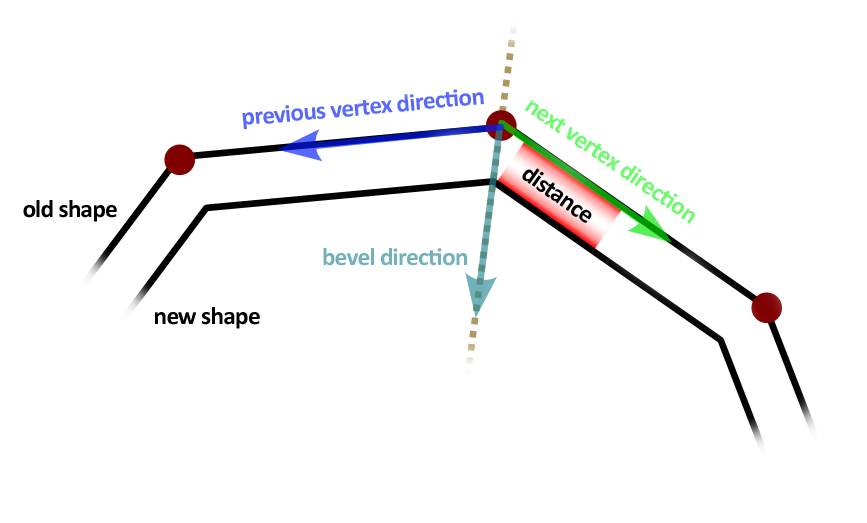
\includegraphics[width=9cm]{gfx/bevel.png}
    \vspace{-1cm}
    \caption{Main directions and relations supporting the bevel operation}
    \label{FIG-GS-BEVEL}
\end{figure}

The algorithm used for beveling faces uses, for each vertex,
the directions from it to the previous and next vertices,
averages it and normalizes it, getting the bevel direction vector with unit length.
The new vertex position is then:

\begin{equation}
	v^{'} = v + b_{dir} \cdot b_{distance}
\end{equation}


\paragraph{Determining Edge Directions}

\begin{figure}[!ht]
    \centering
    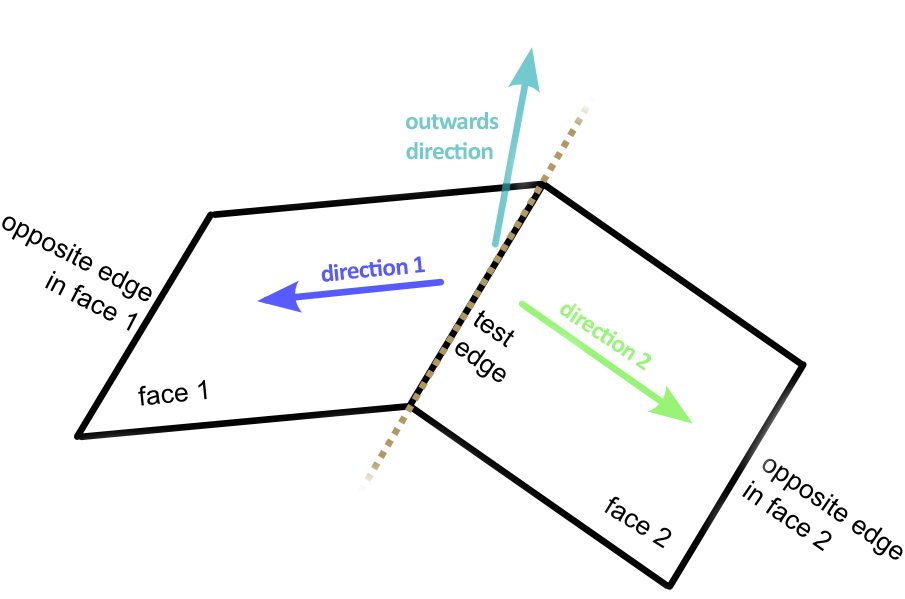
\includegraphics[width=9cm]{gfx/face-dirs.png}
    \vspace{-0.5cm}
    \caption{Determining edge directions from neighboring faces}
    \label{FIG-GS-FACE-DIRS}
\end{figure}

The most relevant directions according to an edge are those along the faces
which share it and the direction farthest away from the other ones.
 
Calculating direction 1 is easy once the edge map is calculated
and getOppositeEdge(edge) function defined.

Direction 2 works the same way, this time following the remaining direction.

The outwards direction resembles the concept of a face normal but applied to an edge
-- it points out relating to the neighboring faces.
This direction can be easily found by averaging the face normals
for the faces containing the selected edge.


\subsection{User Interface}

\emph{Face selection} occurs by drawing a stroke exclusively over a face.

\emph{Edge selection} occurs by crossing the desired edge, with the stroke beginning
on one of its neighboring faces and ending on the remaining one.
Figure \ref{fig:selection} illustrates this procedure.

\begin{figure}[!ht]
	\centering
	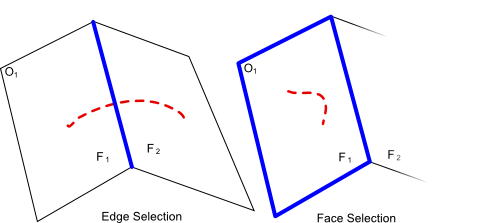
\includegraphics[width=11cm]{gfx/face-edge-selection.png}
	\caption{edge and face selection}
	\label{fig:selection}
\end{figure}

Once the component gets selected, a contextual menu appears in the vicinity
of the selection, allowing the user to select the operation to apply (see figure \ref{fig:contextual}).

\begin{figure}[!ht]
	\centering
	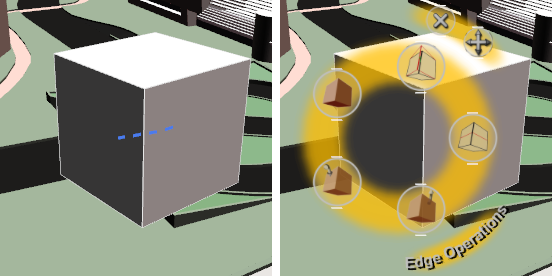
\includegraphics[width=10cm]{gfx/contextual.png}
	\caption{activation of a contextual menu from an edge selection}
	\label{fig:contextual}
\end{figure}

In several of the supported operations one of the parameters is direction.
In those cases the nearest vector direction algorithm is used.
The direction of the ongoing stroke is compared with the set of suggested directions,
with the closest direction being applied in real-time, a mechanism commonly
named \textit{snapping} (see figure \ref{fig:election}).

\begin{figure}[!ht]
	\centering
	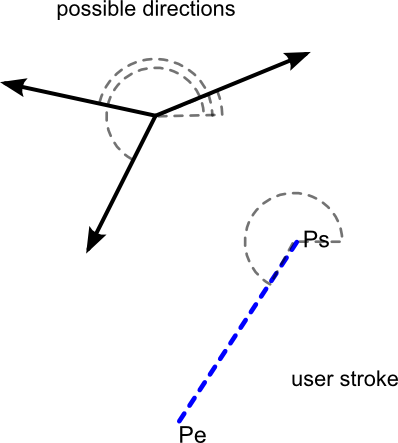
\includegraphics[width=5cm]{gfx/election.png}
	\caption{electing the nearest vector direction}
	\label{fig:election}
\end{figure}

\subsection{Supported Operations}

A description of the supported operations and their provided directions for modification follows,
as seen in figure \ref{fig:shots}.

\begin{figure}[!ht]
	\centering
	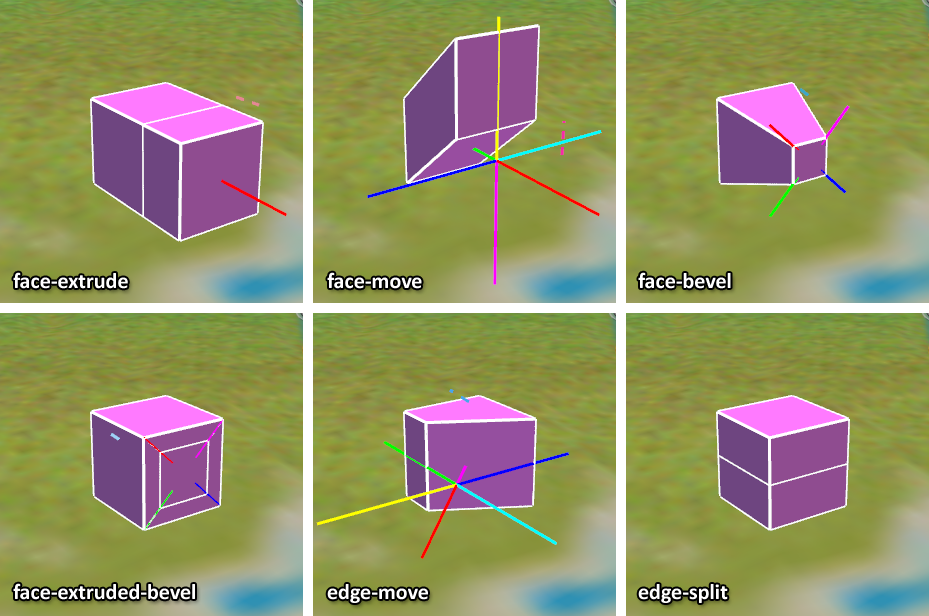
\includegraphics[width=11cm]{gfx/gs-ops.png}
	\caption{geometry manipulation operations}
	\label{fig:shots}
\end{figure}

\subsubsection{Geometry Manipulation Operations}

\begin{description}
	\item[Face Extrude] --
		the direction is extracted from the selected face normal. Displacement based on stroke length.
		
	\item[Face Bevel] --
		the bevel distance depends on the stroke length.
		
	\item[Face Move] --
		this operation supports not only the face normal directions,
		but also the directions from the face center towards the four boundary edges.
		
	\item[Edge Move] --
		supports the edge normal along with the directions from it towards its neighboring faces.
		
	\item[Edge Split] --
		this operation occurs immediately since it doesn't require any real-time input from the user.
		The sketched cut propagates throughout the intrinsic selected face loop, each edge cutting
		the opposite edge in each face of the loop, until either no more faces occur or an already
		visited face is revisited. \TODOL{FIGURE FOR THIS PROCEDURE?}
\end{description}

\subsubsection{Other Operations}

\begin{description}
	\item[Undo] --
		any shape operation previously defined can be reverted.
		
	\item[Loading and Saving] --
		the object can be loaded from or saved to the XML format defined above.
		Exporting content from an external 3D modeler is straightforward.
		An exporting plug-in for Blender was implemented in Python.
\end{description}



%
\section{Custom Scenery Creation Work Flow}

\TODO{blender, XML...}

\TODO{summary of implementation}


